\section{LSTM - Long Short-Term Memory}
\begin{frame}{LSTM - Long Short-Term Memory}
  \LARGE LSTM : \textbf{Long short term memory unit}
\end{frame}

\begin{frame}{LSTM - Long Short-Term Memory}
  \small
  \textbf{Introduced by Hochreiter \& Schmidhuber (1997)}\\[0.8em]
  \textbf{Core Idea:} LSTM uses \textbf{gates} to control what to keep, forget, and output.

  \vspace{1em}
  \textbf{Key Components:}
  \begin{itemize}
    \item[\textcolor{red}{$\blacktriangleright$}] \textbf{Forget Gate} $f_t$
    \item[\textcolor{red}{$\blacktriangleright$}] \textbf{Input Gate} $i_t$
    \item[\textcolor{red}{$\blacktriangleright$}] \textbf{Cell State} $C_t$
    \item[\textcolor{red}{$\blacktriangleright$}] \textbf{Output Gate} $o_t$
  \end{itemize}
\end{frame}

\begin{frame}{LSTM - Long Short-Term Memory}
  \centering
  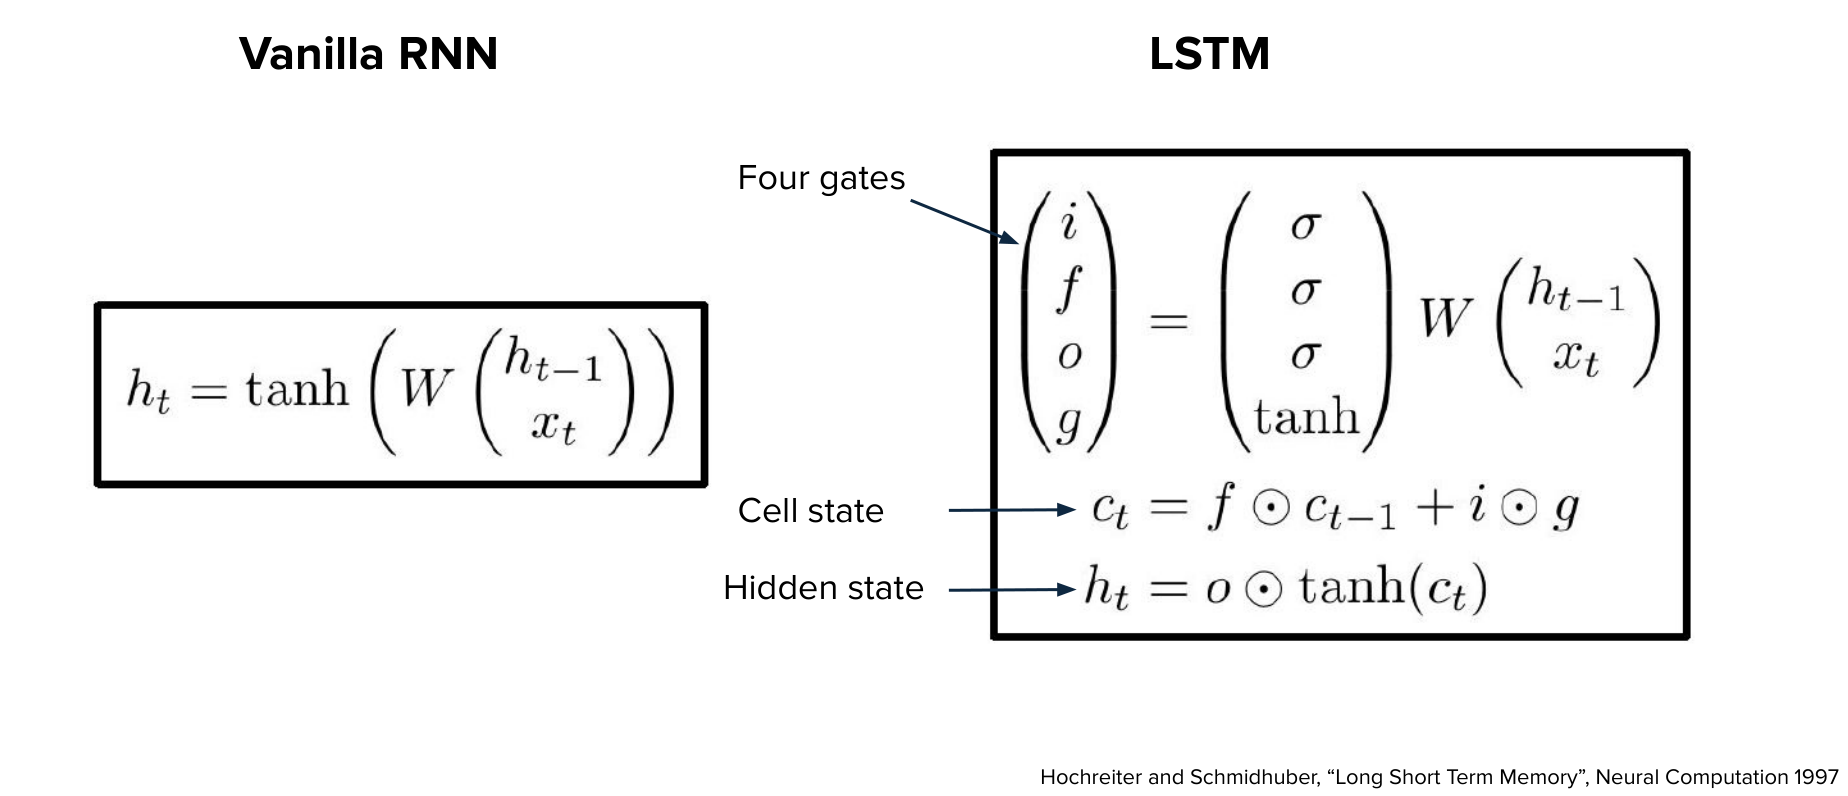
\includegraphics[width=0.9\paperwidth,height=0.95\paperheight,keepaspectratio]{assets/Lecture-3_Recurrent_Neural_Networks/pdf_page_053.png}
\end{frame}

\begin{frame}{LSTM - Long Short-Term Memory: Equations}
  \textbf{Equations:}
  \vspace{0.7em}

  \begin{align*}
    f_t &= \sigma\left(W_f[x_t, h_{t-1}] + b_f\right) \\
    i_t &= \sigma\left(W_i[x_t, h_{t-1}] + b_i\right) \\
    \tilde{C}_t &= \tanh\left(W_c[x_t, h_{t-1}] + b_c\right) \\
    C_t &= f_t * C_{t-1} + i_t * \tilde{C}_t \\
    o_t &= \sigma\left(W_o[x_t, h_{t-1}] + b_o\right) \\
    h_t &= o_t * \tanh\left(C_t\right)
  \end{align*}

  \vspace{1.5em}
  
  {\color{blue} \textbf{Helps retain long-term dependencies}}
\end{frame}

\begin{frame}{LSTMs - A Memorable Solution}
  \begin{itemize}
    \item[$\blacktriangleright$] Learns when to remember and when to forget
    \item[$\blacktriangleright$] \textbf{Basic anatomy:}
      \begin{itemize}
        \item[] \hspace{-1.2em} $\circ$ A cell state
        \item[] \hspace{-1.2em} $\circ$ A hidden state
        \item[] \hspace{-1.2em} $\circ$ Multiple gates
      \end{itemize}
    \vspace{1em}
    \item[$\blacktriangleright$] Gates allow gradients to avoid vanishing and exploding
  \end{itemize}
\end{frame}

\begin{frame}{Long Short-Term Memory}
  \centering
  
\includegraphics[width=0.9\paperwidth,height=0.95\paperheight,keepaspectratio]{assets/Lecture-3_Recurrent_Neural_Networks/pdf_page_056.png}
\end{frame}

\begin{frame}{Long Short-Term Memory}
  \centering
  
\includegraphics[width=0.9\paperwidth,height=0.95\paperheight,keepaspectratio]{assets/Lecture-3_Recurrent_Neural_Networks/pdf_page_057.png}
\end{frame}

\begin{frame}{Long Short-Term Memory}
  \centering
  
\includegraphics[width=0.9\paperwidth,height=0.95\paperheight,keepaspectratio]{assets/Lecture-3_Recurrent_Neural_Networks/pdf_page_058.png}
\end{frame}

\begin{frame}{Long Short-Term Memory}
  \centering
  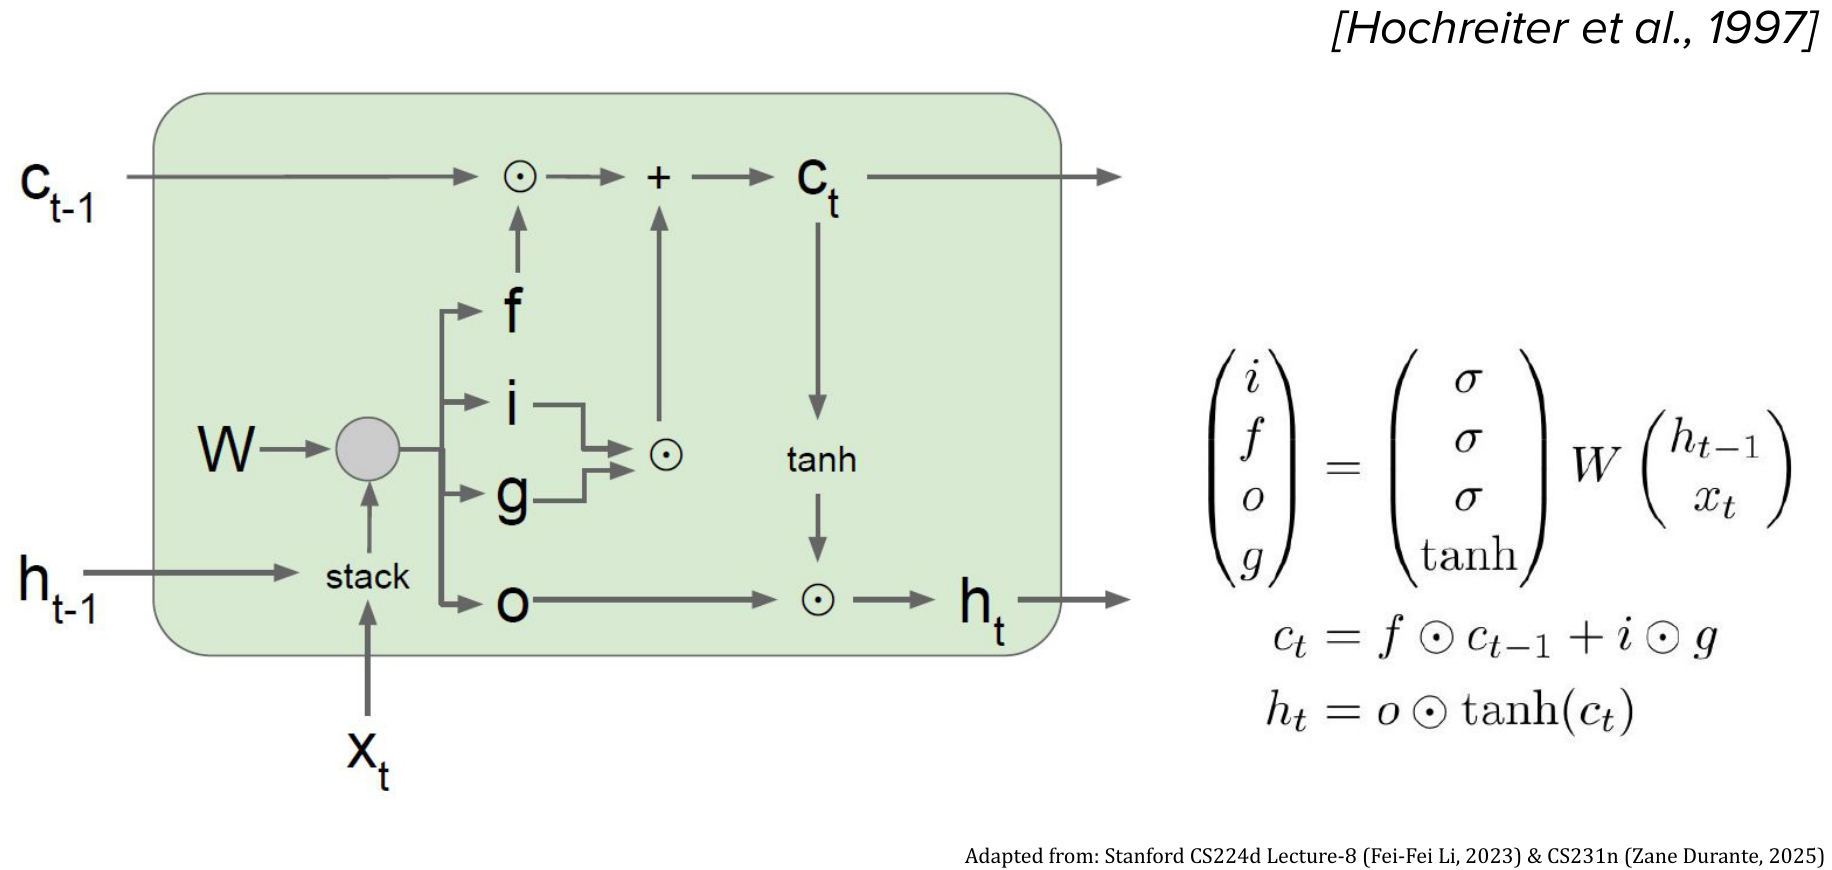
\includegraphics[width=0.9\paperwidth,height=0.95\paperheight,keepaspectratio]{assets/Lecture-3_Recurrent_Neural_Networks/pdf_page_059.png}
\end{frame}

\begin{frame}{Gates in LSTM}
  \centering
  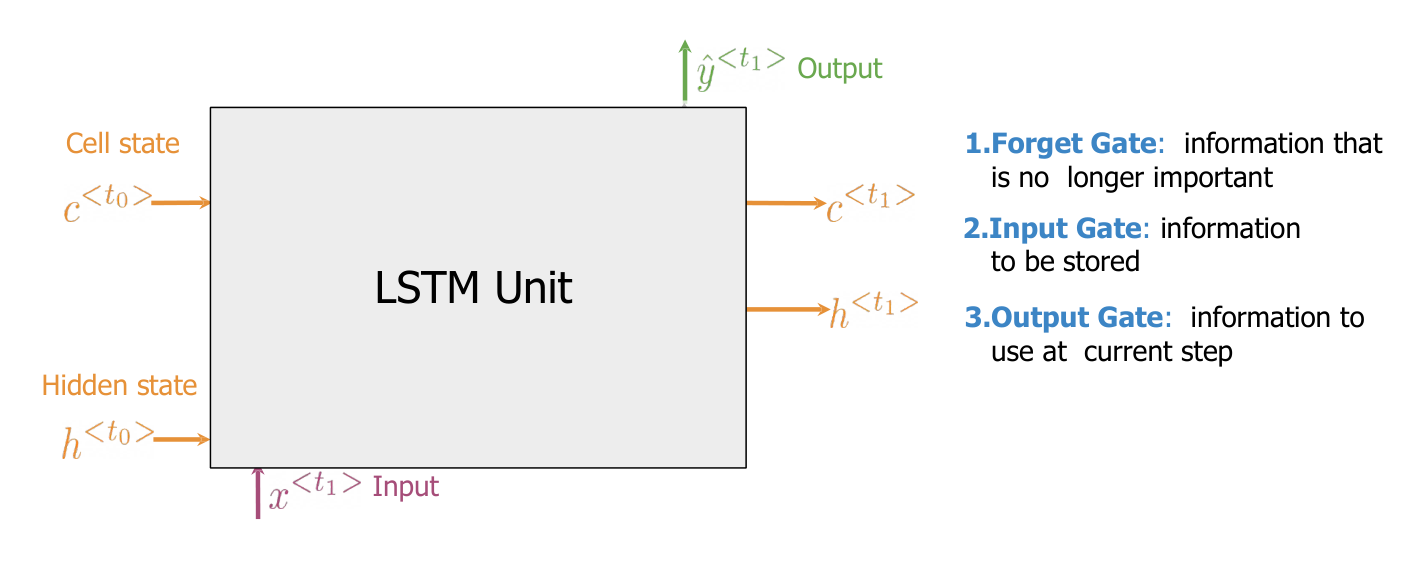
\includegraphics[width=0.9\paperwidth,height=0.95\paperheight,keepaspectratio]{assets/Lecture-3_Recurrent_Neural_Networks/pdf_page_060.png}
\end{frame}

\begin{frame}{Gates in LSTM}
  \centering
  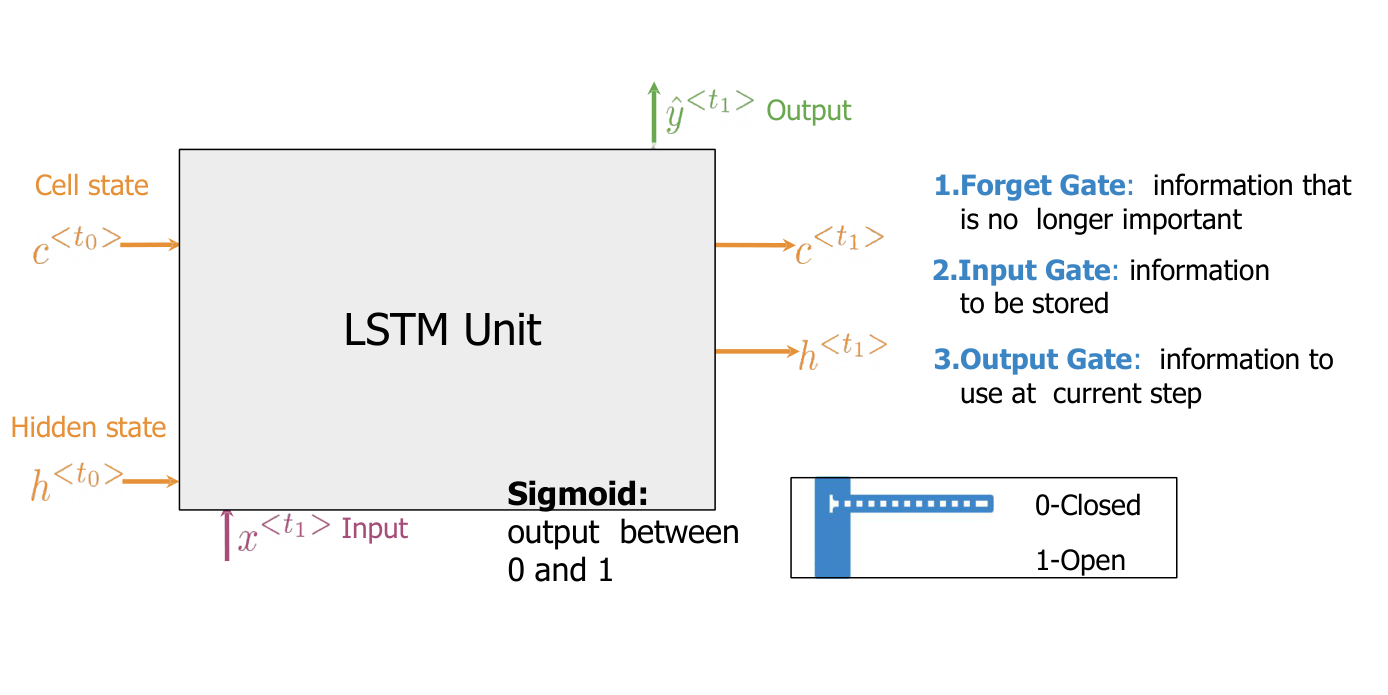
\includegraphics[width=0.9\paperwidth,height=0.95\paperheight,keepaspectratio]{assets/Lecture-3_Recurrent_Neural_Networks/pdf_page_061.png}
\end{frame}

\begin{frame}{Candidate Cell State}
  \centering
  
\includegraphics[width=0.9\paperwidth,height=0.95\paperheight,keepaspectratio]{assets/Lecture-3_Recurrent_Neural_Networks/pdf_page_062.png}
\end{frame}

\begin{frame}{New Cell State}
  \centering
  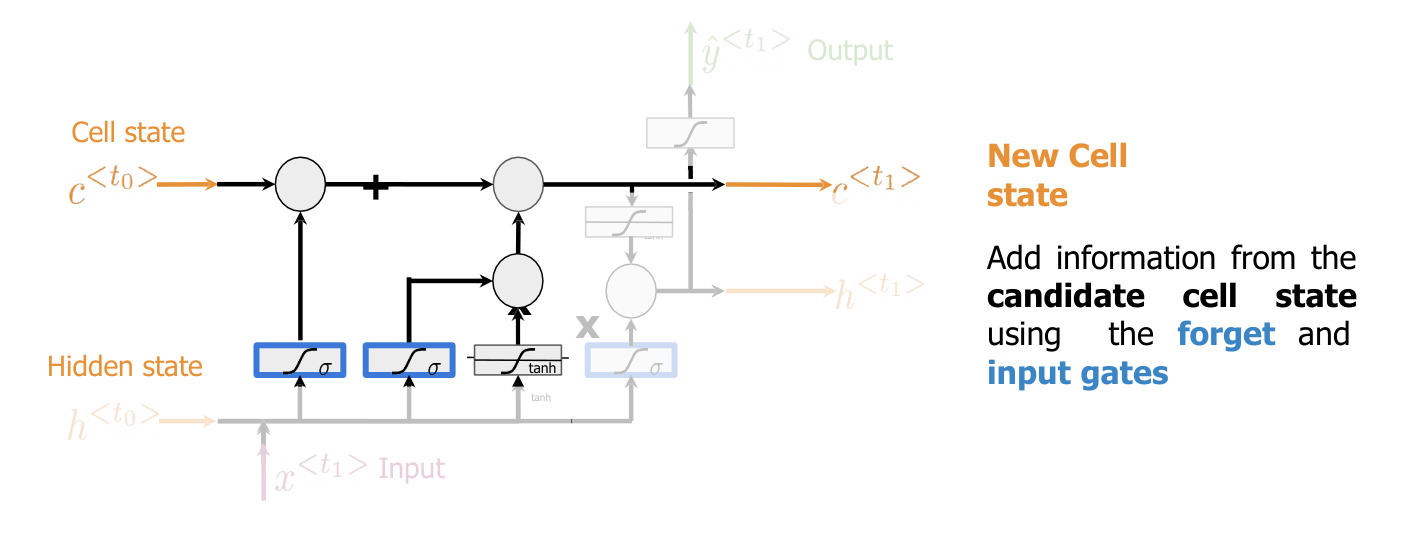
\includegraphics[width=0.9\paperwidth,height=0.95\paperheight,keepaspectratio]{assets/Lecture-3_Recurrent_Neural_Networks/pdf_page_063.png}
\end{frame}

\begin{frame}{New Hidden State}
  \centering
  
\includegraphics[width=0.9\paperwidth,height=0.95\paperheight,keepaspectratio]{assets/Lecture-3_Recurrent_Neural_Networks/pdf_page_064.png}
\end{frame}

\begin{frame}{LSTM: Gradient Flow}
  \centering
  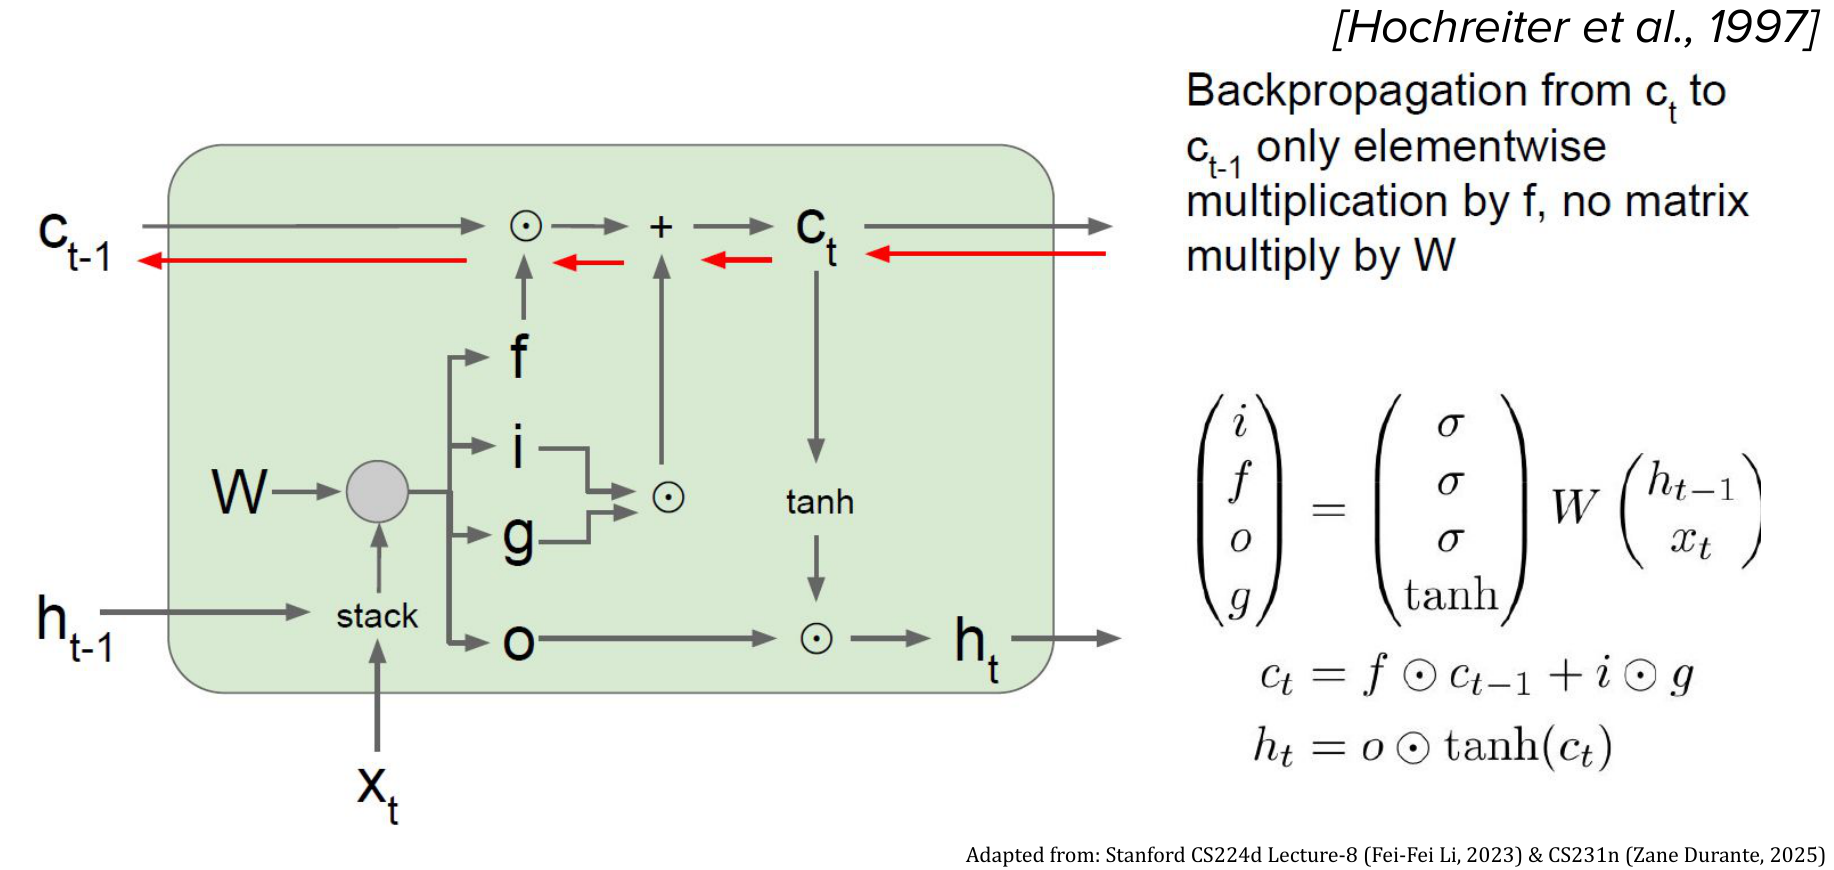
\includegraphics[width=0.9\paperwidth,height=0.95\paperheight,keepaspectratio]{assets/Lecture-3_Recurrent_Neural_Networks/pdf_page_065.png}
\end{frame}

\begin{frame}{LSTM: Gradient Flow}
  \centering
  
\includegraphics[width=0.9\paperwidth,height=0.95\paperheight,keepaspectratio]{assets/Lecture-3_Recurrent_Neural_Networks/pdf_page_066.png}
\end{frame}

\begin{frame}{LSTM: Gradient Flow}
  \centering
  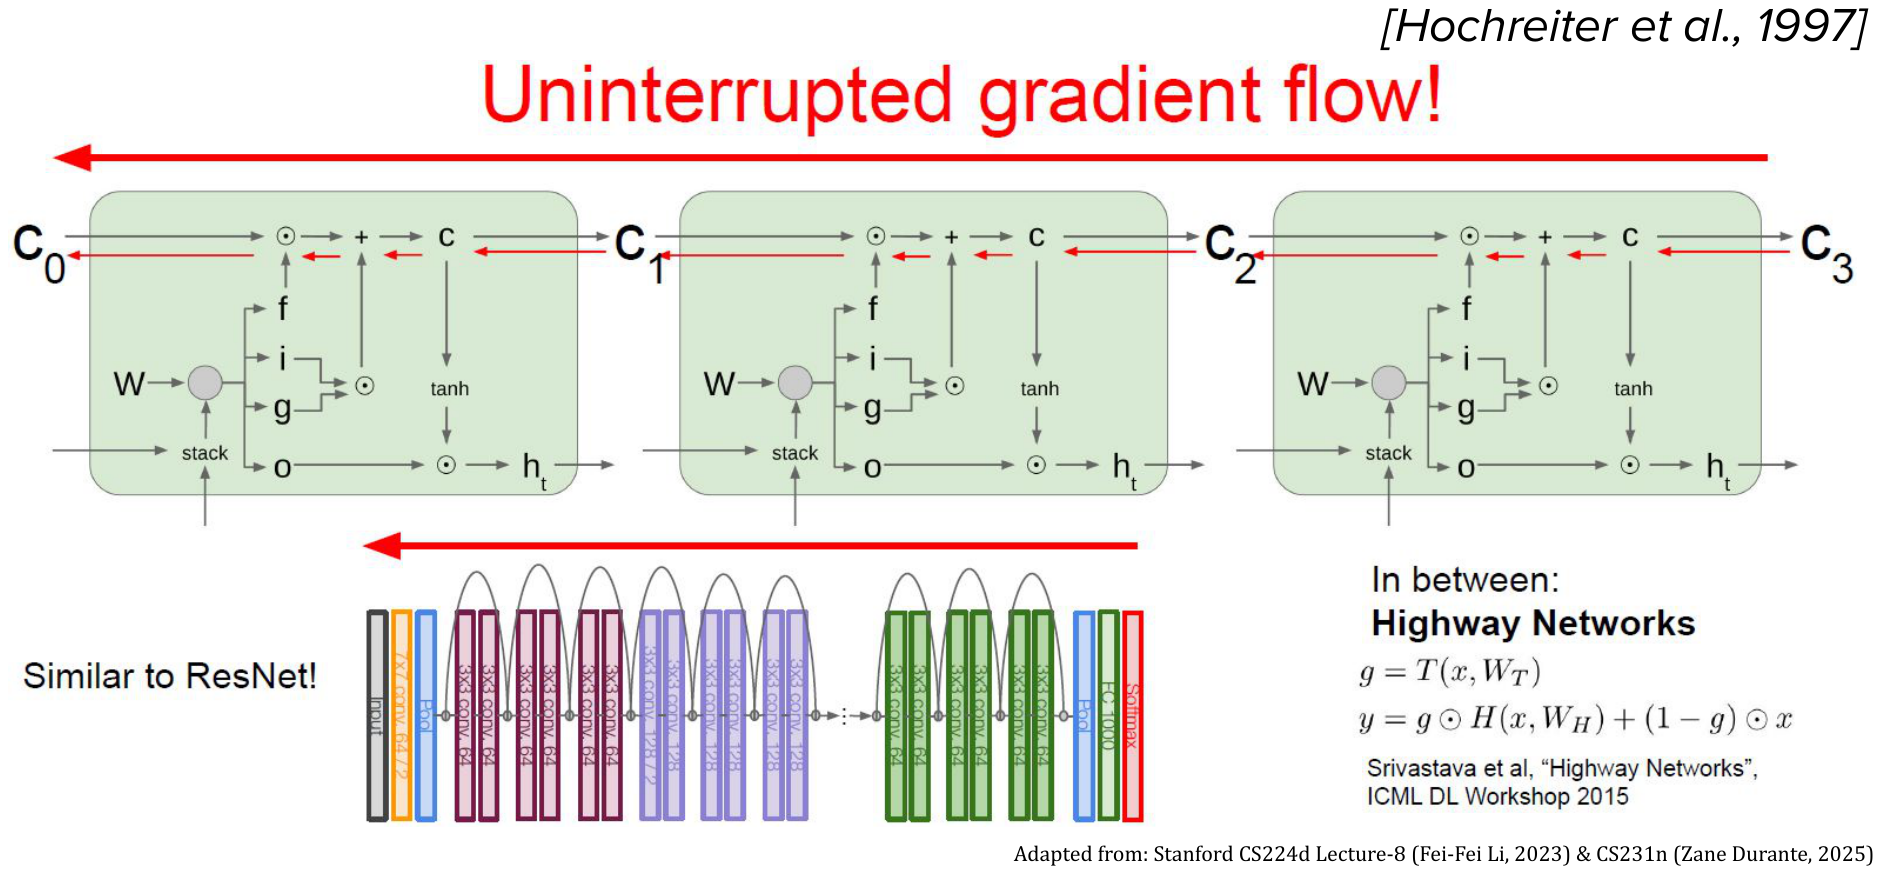
\includegraphics[width=0.9\paperwidth,height=0.95\paperheight,keepaspectratio]{assets/Lecture-3_Recurrent_Neural_Networks/pdf_page_067.png}
\end{frame}

\begin{frame}{Do LSTMs solve the vanishing gradient problem?}
  \begin{itemize}
    \item The LSTM architecture makes it easier for the RNN to preserve information over many timesteps.
    \begin{itemize}
      \item e.g.\ if the forget gate $f = 1$ and input gate $i = 0$, then the information of that cell is preserved indefinitely.
      \item By contrast, it is harder for a vanilla RNN to learn a recurrent weight matrix $W_h$ that preserves information in the hidden state.
    \end{itemize}
    \item LSTM \textcolor{red}{\textbf{doesn't guarantee}} that there is no vanishing/exploding gradient, but it does provide an easier way for the model to learn long-distance dependencies.
  \end{itemize}
\end{frame}
